
\documentclass[final]{beamer}

\usepackage[scale=1.24]{beamerposter} % Use the beamerposter package for laying out the poster

\usetheme{confposter} % Use the confposter theme supplied with this template

\setbeamercolor{block title}{fg=ngreen,bg=white} % Colors of the block titles
\setbeamercolor{block body}{fg=black,bg=white} % Colors of the body of blocks
\setbeamercolor{block alerted title}{fg=white,bg=dblue!70} % Colors of the highlighted block titles
\setbeamercolor{block alerted body}{fg=black,bg=dblue!10} % Colors of the body of highlighted blocks
% Many more colors are available for use in beamerthemeconfposter.sty

%-----------------------------------------------------------
% Define the column widths and overall poster size
% To set effective sepwid, onecolwid and twocolwid values, first choose how many columns you want and how much separation you want between columns
% In this template, the separation width chosen is 0.024 of the paper width and a 4-column layout
% onecolwid should therefore be (1-(# of columns+1)*sepwid)/# of columns e.g. (1-(4+1)*0.024)/4 = 0.22
% Set twocolwid to be (2*onecolwid)+sepwid = 0.464
% Set threecolwid to be (3*onecolwid)+2*sepwid = 0.708

\newlength{\sepwid}
\newlength{\onecolwid}
\newlength{\twocolwid}
\newlength{\threecolwid}
\setlength{\paperwidth}{48in} % A0 width: 46.8in
\setlength{\paperheight}{36in} % A0 height: 33.1in
\setlength{\sepwid}{0.024\paperwidth} % Separation width (white space) between columns
\setlength{\onecolwid}{0.30\paperwidth} % Width of one column
\setlength{\twocolwid}{0.62\paperwidth} % Width of two columns
% \setlength{\threecolwid}{0.708\paperwidth} % Width of three columns
\setlength{\topmargin}{-0.5in} % Reduce the top margin size
%-----------------------------------------------------------

\usepackage{graphicx}  % Required for including images

\usepackage{booktabs} % Top and bottom rules for tables

%----------------------------------------------------------------------------------------
%	TITLE SECTION 
%----------------------------------------------------------------------------------------

\title{ETERNITY: FUNCTIONS, F4: Logarithm} % Poster title

\author{SOEN 6011, Team C, Student N4, Kenlo DINH VAN} % Author(s)

\institute{August, 12\superscript{th} ,2019} % Institution(s)

%----------------------------------------------------------------------------------------

\begin{document}

\addtobeamertemplate{block end}{}{\vspace*{2ex}} % White space under blocks
\addtobeamertemplate{block alerted end}{}{\vspace*{2ex}} % White space under highlighted (alert) blocks

\setlength{\belowcaptionskip}{2ex} % White space under figures
\setlength\belowdisplayshortskip{2ex} % White space under equations

\begin{frame}[t] % The whole poster is enclosed in one beamer frame

\begin{columns}[t] % The whole poster consists of three major columns, the second of which is split into two columns twice - the [t] option aligns each column's content to the top

\begin{column}{\sepwid}\end{column} % Empty spacer column

\begin{column}{\onecolwid} % The first column

%----------------------------------------------------------------------------------------
%	SUMMARY
%----------------------------------------------------------------------------------------

\begin{alertblock}{Retrospective's Summary}
\begin{itemize}
\item Function Description.
\item Important Properties.
\item Project's Decisions.
\item Code Review.
\item Testing.
% \item Conclusion.
\end{itemize}

\end{alertblock}

%----------------------------------------------------------------------------------------
%	Function Description
%----------------------------------------------------------------------------------------

\begin{block}{Logarithms}

\textbf{Quick Facts}
\begin{itemize}
\item introduced by \textbf{John Napier} in 1614.
\item \textbf{inverse} function to \textbf{exponentiation}, y = x as axis of symmetry.
\item $log_b(x) = y$ can be read: \textbf{x} equals \textbf{base b} to the \textbf{power y}.
\item commonly used logarithms: \textbf{binary} (b = 2), \textbf{natural} (b = e), \textbf{common} (b = 10).
\item variable \textbf{x} {\textgreater} 0 (in \textbf{R}).
\item base \textbf{b} ${\neq}$ 1 and b {\textgreater} 0 (in \textbf{R}).
\item co-domain: real numbers \textbf{R}.

\end{itemize}

\textbf{Base b}\\*
\textbf{b} determines the behaviour of the logarithm:
\begin{itemize}
\item $x\in(0;1)$ decreasing function.
\item $x\in(1; +\infty)$ increasing function.
\end{itemize}

\textbf{Graph of Logarithmic Functions}
\end{block}
%------------------------------------------------

\begin{figure}
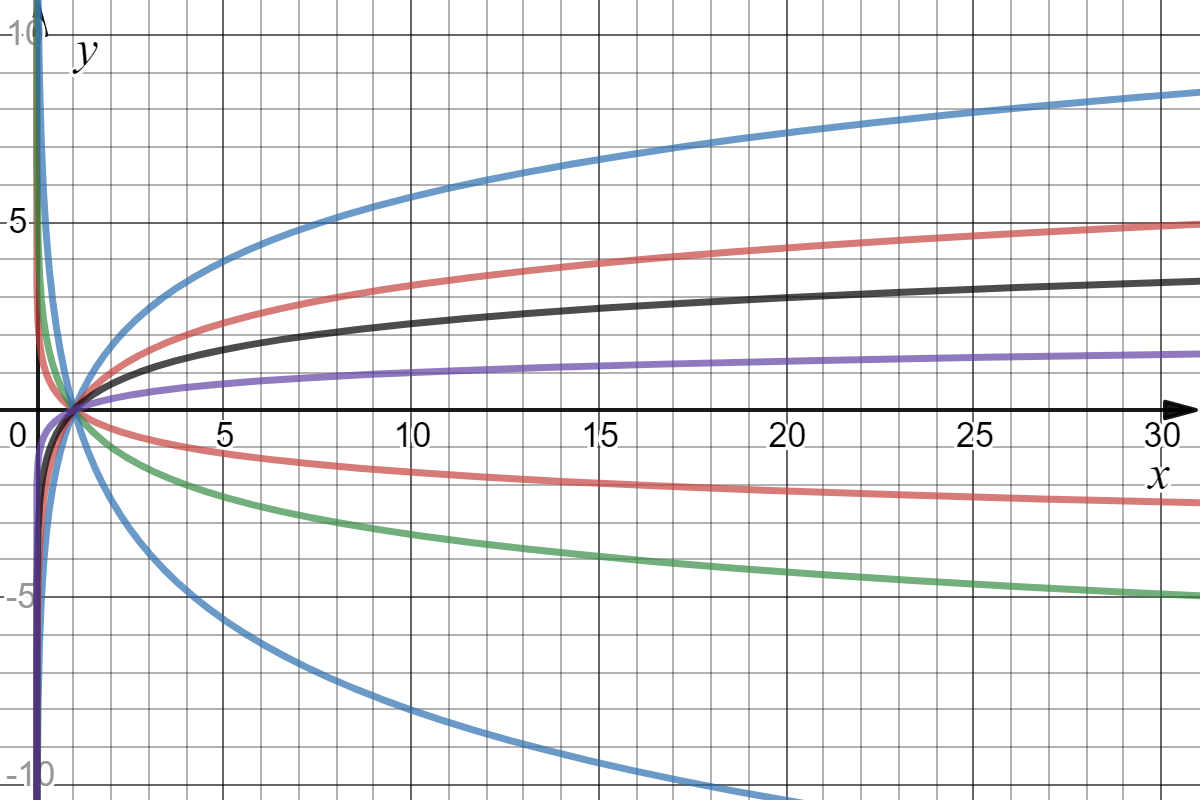
\includegraphics[width=1\linewidth]{m_rec_m.png}
\caption{Graph of $f(x)=log_{\{1.5, 2, e, 10, 0.25, 0.5, 0.75\}}(x)$}
\end{figure}

%----------------------------------------------------------------------------------------

\end{column} % End of the first column

\begin{column}{\sepwid}\end{column} % Empty spacer column

\begin{column}{\twocolwid} % Begin a column which is two columns wide (column 2)

\begin{columns}[t,totalwidth=\twocolwid] % Split up the two columns wide column

\begin{column}{\onecolwid}\vspace{-.6in} % The first column within column 2 (column 2.1)

%----------------------------------------------------------------------------------------
%	Important Properties
%----------------------------------------------------------------------------------------

\begin{block}{Important properties}

\textbf{Change of base:}\\*
\begin{equation*}
 \log _{b}x={\frac {\log _{k}x}{\log _{k}b}}\
\end{equation*} 
\\
\textbf{Natural Logarithm identity:}\\*
\begin{equation*}
\ln(x)\ =\ \lim_{n\rightarrow\infty}\ n{\ (\ x^{1/n}\ }-\ 1)
\end{equation*}
\end{block}
Those properties were crucial in implementing the logarithmic function.\\
We first approximate ln(x), then convert it to the desired base.

%----------------------------------------------------------------------------------------

\end{column} % End of column 2.1

\begin{column}{\onecolwid}\vspace{-.6in} % The second column within column 2 (column 2.2)

%----------------------------------------------------------------------------------------
%	P
%----------------------------------------------------------------------------------------

\begin{block}{Critical Decisions}
1. Algorithm Selection: ln(x) approximation\\
Trade-offs: ease of implementation and efficiency versus accuracy.
Allowed function development within the project's time constraints.
\[\]
2. Coding Style: Google Java Style Guide.\\
Inner-team coding style uniformity, favored readable and predictable code.
Wide range of tools and example available.
\[\]
3. Tools Selection:\\
The set of tools used during this project eased the development process, as well as helped time efficiency.
LaTex editor: Overleaf, VCS: GitHub.
IDE: Jetbrains IntelliJ, CheckStyle, JUnit, Reviewable.

\end{block}

%----------------------------------------------------------------------------------------

\end{column} % End of column 2.2

\end{columns} % End of the split of column 2 - any content after this will now take up 2 columns width

%----------------------------------------------------------------------------------------
%	IMPORTANT To REMEMBER
%----------------------------------------------------------------------------------------

\begin{alertblock}{Lessons Learned}

The reviewing and testing experiences of this project has allowed us to extract the following lessons.

\end{alertblock} 

%----------------------------------------------------------------------------------------

\begin{columns}[t,totalwidth=\twocolwid] % Split up the two columns wide column again

\begin{column}{\onecolwid} % The first column within column 2 (column 2.1)

%----------------------------------------------------------------------------------------
%	Code Review
%----------------------------------------------------------------------------------------

\begin{block}{Code Review}
\begin{itemize}
\item Code review is simpler when \textbf{VCS} resources are properly managed, allows seamless integration with code review tools and git features. (branches, pull requests)
\[\]
\item Code review is more efficient when the \textbf{coding style} is uniform and predictable within a team, peer reviewers read and understand the code faster.
\[\]
\item Choosing the right \textbf{code review tools} allows spending less efforts in sometimes tedious tasks.
\[\]
\item Bad practice: sharing compressed source code. Time wasted in importing and configuring projects, absence of version history.
\end{itemize}
\end{block}

%----------------------------------------------------------------------------------------

\end{column} % End of column 2.1

\begin{column}{\onecolwid} % The second column within column 2 (column 2.2)

%----------------------------------------------------------------------------------------
%	Testing
%----------------------------------------------------------------------------------------

\begin{block}{Testing}
\begin{itemize}
\item \textbf{Functional Requirements} should have been formulated in concert \textbf{with the team} for homogeneous requirements (existence of common requirements, as well as better, project-wide, requirement identifiers).
\[\]
\item All Unit tests should have been written with the \textbf{same version} of a \textbf{unit test framework} (ex: JUnit 4 or 5), a lot of time was spent on adjusting configuration, \textbf{dependencies}.
\[\]
\item A \textbf{common unit testing guide line} should have been selected by the whole team. (disparate unit testing practices among team members)

\end{itemize}

\end{block}

\begin{block}{Repository}
All project artifacts are available on GitHub
\begin{itemize}
\item https://github.com/k3nlo/SOEN6011\_TeamC\_N4
\end{itemize}

\end{block}



%----------------------------------------------------------------------------------------

\end{column} % End of column 2.2

\end{columns} % End of the split of column 2

\end{column} % End of the second column

\begin{column}{\sepwid}\end{column} % Empty spacer column

\begin{column}{\onecolwid} % The third column

%----------------------------------------------------------------------------------------
%	CONCLUSION
%----------------------------------------------------------------------------------------

% \begin{block}{Vieta's Formulas- Task}
% 1. Prove that $$x_1x_2 = \frac{c}{a}$$
% \[\]
% \[\]
% \[\]
% \[\]
% \[\]

% \end{block}


%----------------------------------------------------------------------------------------
%	ACKNOWLEDGEMENTS
%----------------------------------------------------------------------------------------

% \setbeamercolor{block title}{fg=red,bg=white} % Change the block title color

% \begin{block}{Glossary}

% \begin{table}
% \vspace{2ex}
% \begin{tabular}{l l l l}
% \toprule
% \textbf{verb} & \textbf{noun} & \textbf{meaning}\\
% \midrule
% add & addition & $+$ \\
% subtract & subtraction & $-$ \\
% multiply & multiplication & $\cdot$ \\
% divide & division & $\div$ \\
% solve & solution & getting answer \\
% substitute & substitution & $t=x^2$ \\



% \bottomrule
% \end{tabular}
% \caption{Word Formation}
% \end{table}


% \end{block}

% \setbeamercolor{block alerted title}{fg=black,bg=norange} % Change the alert block title colors
% \setbeamercolor{block alerted body}{fg=black,bg=white} % Change the alert block body colors

% \begin{alertblock}{Some Necessary and Useful Vocabulary}

% \begin{itemize}
% \item (n.) sign $\rightarrow$ $+$ or $-$
% \item (n.) equation $\rightarrow something = 0$ 
% \item (n.) factor $\rightarrow$ two multiplied factors give result
% \item (v.) factorise $\rightarrow$ putting into brackets
% \item (n.) coefficient $\rightarrow$ a constant number i.e. $a$, $b$, $c$ in a pattern $ax^2+bx+c$
% \item (n.) quadratic function $\rightarrow$ $f(x) = ax^2+bx+c$
% \item (n.) root $\rightarrow$ $\sqrt{sth}$ or solution of quadratic equation
% \item (n.) formula $=$ pattern
% \end{itemize}

% \end{alertblock}


%----------------------------------------------------------------------------------------

\end{column} % End of the third column

\end{columns} % End of all the columns in the poster

\end{frame} % End of the enclosing frame

\end{document}
